
Once the plane-wave expansions are formed for each of the FGT boxes, step (ii)
involves translating the information to its interaction list to obtain the
local expansions. A direct scheme forms the local expansions by simply visiting
all the boxes in $\mathcal{I}|B|$ for each box $B$ and translating the wave
expansions according to (\ref{e:w2l}). Since the size of the interaction list
is $K^d$, this algorithm requires $\mathcal{O}(K^dp^d|B|)$ work to form all
local expansions, where $|B|$ is the total number of boxes. By using the
sweeping algorithm proposed in \cite{fggt}, the complexity of this step can be
reduced to $\mathcal{O}(3dp^d|B|)$. This algorithm is optimal in terms of work,
but is not ideal in terms of storage. In cases where we have non-uniform
distributions (resulting in several empty boxes), the sweep algorithm requires
storage at all boxes $B_i$, till the sweeps in all $d$ dimensions are
completed. We propose a new algorithm for accelerating the plane-wave
translations, which only needs $\mathcal{O}(|B|^\frac{d-1}{d})$ storage instead
of $\mathcal{O}(|B|)$ storage as required by the sweeping algorithm from
\cite{fggt}. In addition, the algorithm is work optimal for distributions with
\ul{distribution density} less than $60\%$ (for $d=3$).

\subsection{Accelerating the plane-wave translation step}
The sweeping algorithm discussed in \cite{fggt} reduces this cost to $\bigO(9 p^3 N_B)$. 
This algorithm is however not memory efficient when there are ``holes'' in the domain. We propose the following modification which has a much smaller memory footprint.

\begin{itemize}
\item First compute the local expansions at the outermost layer of the FGT boxes. These are shown in Figure \ref{fig:outer} in orange. It is possible to speed up this initial computation as well since we can compute the local expansions for a small number of boxes and use the propagation rule.
\item We propagate the local expansions from this initial layer to subsequent layers. The main task is to understand this propagation. Consider the case shown in Figure \ref{fig:corner} where we need to compute the local expansion of the Green box ( $B(i+1,j+1)$), given the local expansions of the adjacent boxes (in Orange).
\item The local expansion $v_k^{B(i+1, j+1)}$ can be written in terms for the local expansions of $B(i,j), B(i+1,j)$ and $B(i,j+1)$, along with the corner box which is in the influence list of $B(i+1, j+1)$ but not of the others ($+$) and the box which is in the influence list of $B(i,j)$ but not of the other three($-$). This is marked in Figure \ref{fig:corner} assuming $K=3, n=1$. The local expansion is given by,
\[
	v_k^{i+1,j+1} = e^{iz_k s/\sqrt{\delta}} v_k^{i+1,j} + e^{iz_k s/\sqrt{\delta}} v_k^{i,j+1}
					- e^{iz_k s/\sqrt{\delta}} v_k^{i,j} - e^{iz_k ns/\sqrt{\delta}} w_k^{i+n+1,j+n+1} + e^{-iz_k ns/\sqrt{\delta}} w_k^{i-n,j-n}
\]
\item The propagation can then be used to propagate to the remaining boxes in the new propagation layer. At any given stage only the values of the propagation layer needs to be stored. The values of any non-zero FGT boxes doesn't need to be remembered.

\end{itemize}

\begin{figure}[h]
\centering
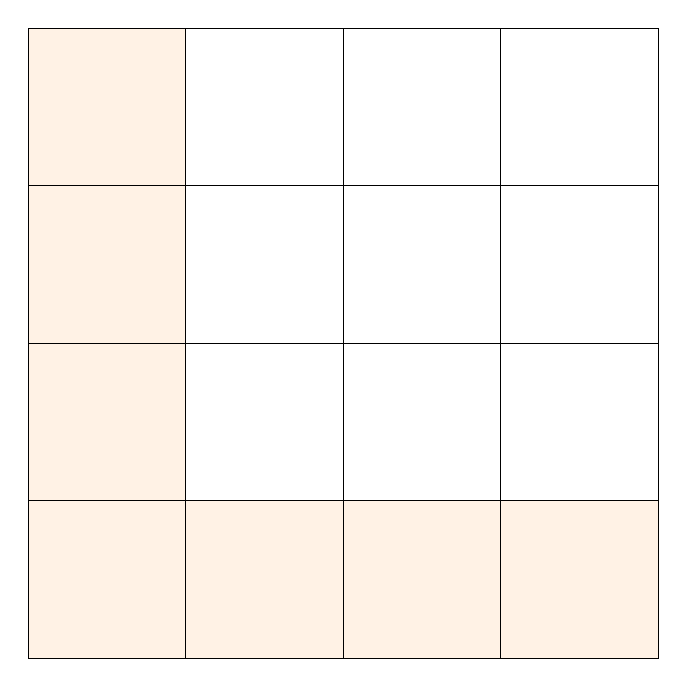
\begin{tikzpicture}
	
	\draw[fill=orange!10] (0,0) rectangle +(8,2);
	\draw[fill=orange!10] (0,2) rectangle +(2,6);
		
	% the grid ...
	\draw[step=2cm] (0,0) grid (8,8);	
	
\end{tikzpicture}
\caption{\small The outermost layer, for which the local expansions are computed directly. 
}
\label{fig:outer}
\end{figure}



\begin{figure}[h]
\centering
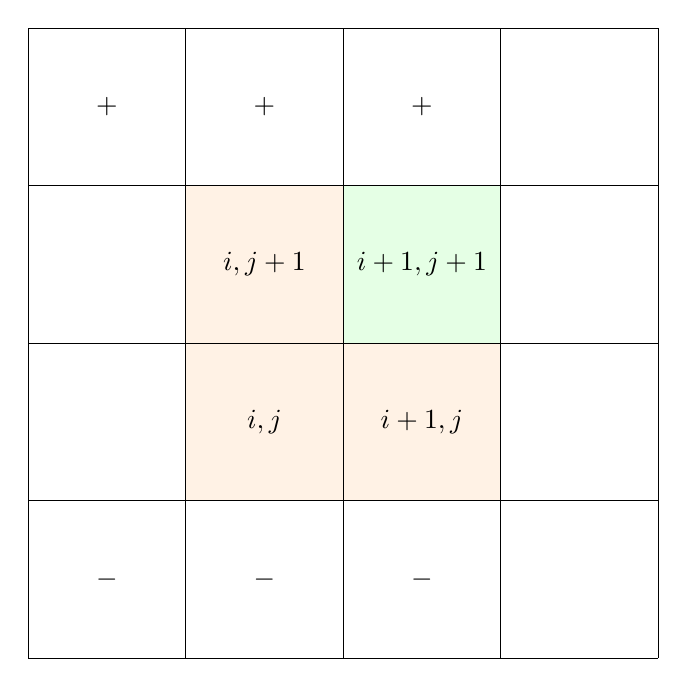
\begin{tikzpicture}
	
	\draw[fill=orange!10] (2,2) rectangle +(4,2);
	\draw[fill=orange!10] (2,2) rectangle +(2,4);
	
	\draw[fill=green!10] (4,4) rectangle +(2,2);		
	% the grid ...
	\draw[step=2cm] (0,0) grid (8,8);	
	
	\draw (3,3) node {$i, j$};
	\draw (5,3) node {$i+1, j$};
	\draw (3,5) node {$i, j+1$};
	\draw (5,5) node {$i+1, j+1$};
	
	\draw (1,1) node {$-$};
	\draw (3,1) node {$-$};
	\draw (5,1) node {$-$};
	
	\draw (1,7) node {$+$};
	\draw (3,7) node {$+$};
	\draw (5,7) node {$+$};
\end{tikzpicture}
\caption{\small The Contributions. 
}
\label{fig:corner2}
\end{figure}


\begin{figure}[h]
\centering
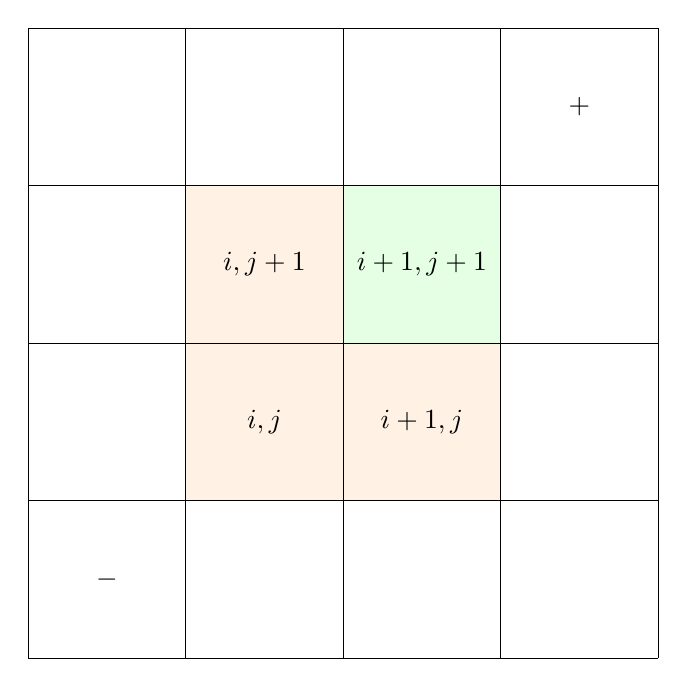
\begin{tikzpicture}
	
	\draw[fill=orange!10] (2,2) rectangle +(4,2);
	\draw[fill=orange!10] (2,2) rectangle +(2,4);
	
	\draw[fill=green!10] (4,4) rectangle +(2,2);		
	% the grid ...
	\draw[step=2cm] (0,0) grid (8,8);	
	
	\draw (3,3) node {$i, j$};
	\draw (5,3) node {$i+1, j$};
	\draw (3,5) node {$i, j+1$};
	\draw (5,5) node {$i+1, j+1$};
	
	\draw (1,1) node {$-$};
	\draw (7,7) node {$+$};
			
\end{tikzpicture}
\caption{\small The propagation of the local expansions using neighbors. 
}
\label{fig:corner}
\end{figure}


